% ~ 6 pages
\chapter{Machine Learning}
\label{sec:ml}

\begin{itemize}
\item Supervised learning
\item Classification
\item Over-fitting
\end{itemize}

\section{Boosted Decision Trees}
\label{sec:bdt}

\todo{Focus on classification with two classes}

\begin{itemize}
\item Tree-based model: recursively partition input space into subregions via
  binary splits on the coordinate axes (parallel to the coordinate axes) of the
  input space until some stopping criterion is fulfilled (description by a
  binary tree)
\item Dataflow: top of the tree - full population; subsets of the full
  population at deeper levels
\item Training: Greedy -- look for best (according to some loss) split in all
  variables and repeat for subregions
\item Impurity measure: Gini index (or Gini impurity): $2 p (1 - p)$ where $p$
  is the signal purity in a region (splits that split off pure background as
  well as signal are equivalent). Probability to assign the correct label to a
  randomly picked observation when randomly assigning according to the
  distribution of labels in the sample.
\item The split has to be weighted by the weight of events in each subregion:
  \begin{align*}
    \frac{w_\mathrm{L} \times 2 p_\mathrm{L} (1 - p_\mathrm{L}) + w_\mathrm{R} \times 2 p_\mathrm{R} (1 - p_\mathrm{R})}{w_\mathrm{L} + w_\mathrm{R}}
  \end{align*}
  weighted average of the Gini impurity of both subregions
\item Each subregion is assigned the majority class or the signal purity in that region
\end{itemize}

Keep this short!

Elements of statistical learning \cite{esl}

\begin{itemize}
\item Boosting: Adaptive Boosting $\alpha$, Gradient Boosting $\eta$
\item Node splitting: Gini Index
\item Hyperparameters: $N_\mathrm{Trees}$, $d_\mathrm{Tree}$,
\end{itemize}

\section{Neural Networks}
\label{sec:nn}

\todo{Explain notation -- bold for vectors and matrices}

\subsection{Feedforward Neural Networks}
\label{sec:nn_feedforward}

\begin{figure}[ht]
  \begin{subfigure}[t]{0.55\textwidth}
    \centering
    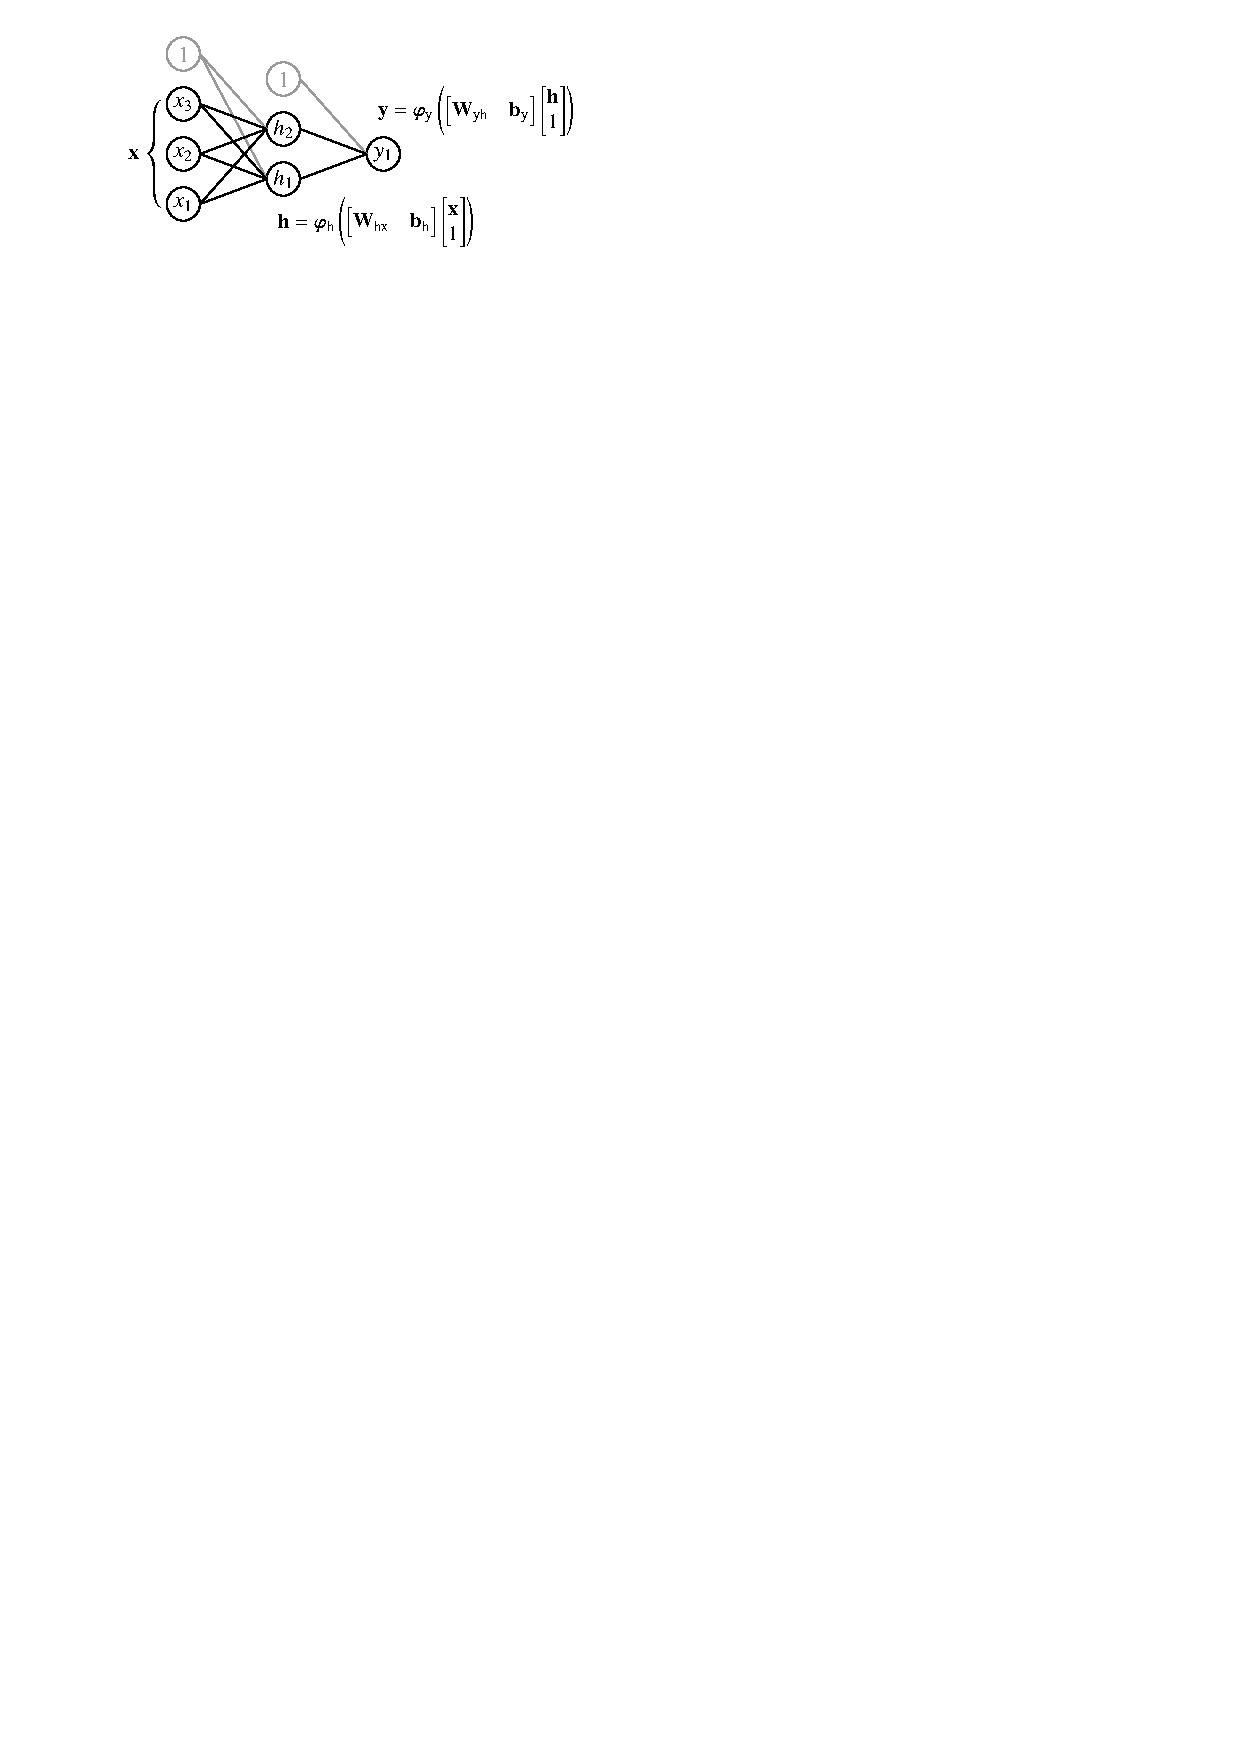
\includegraphics{./figures/theory/mlp.pdf}
    \subcaption{Schematic depiction of a multi-layer perceptron with input
      neurons $\mathbf{x}$, hidden layer activation $\mathbf{h}$ and output
      activation $\mathbf{y}$. The layers are connected via weight matrices
      $\mathbf{W}$ and optional bias vectors $\mathbf{b}$. Neuron activations
      are given after applying an element-wise activation function $\bm{\varphi}$.}
    \label{fig:multi_layer_perceptron}
  \end{subfigure}\hfill
  \begin{subfigure}[t]{0.4\textwidth}
    \centering
    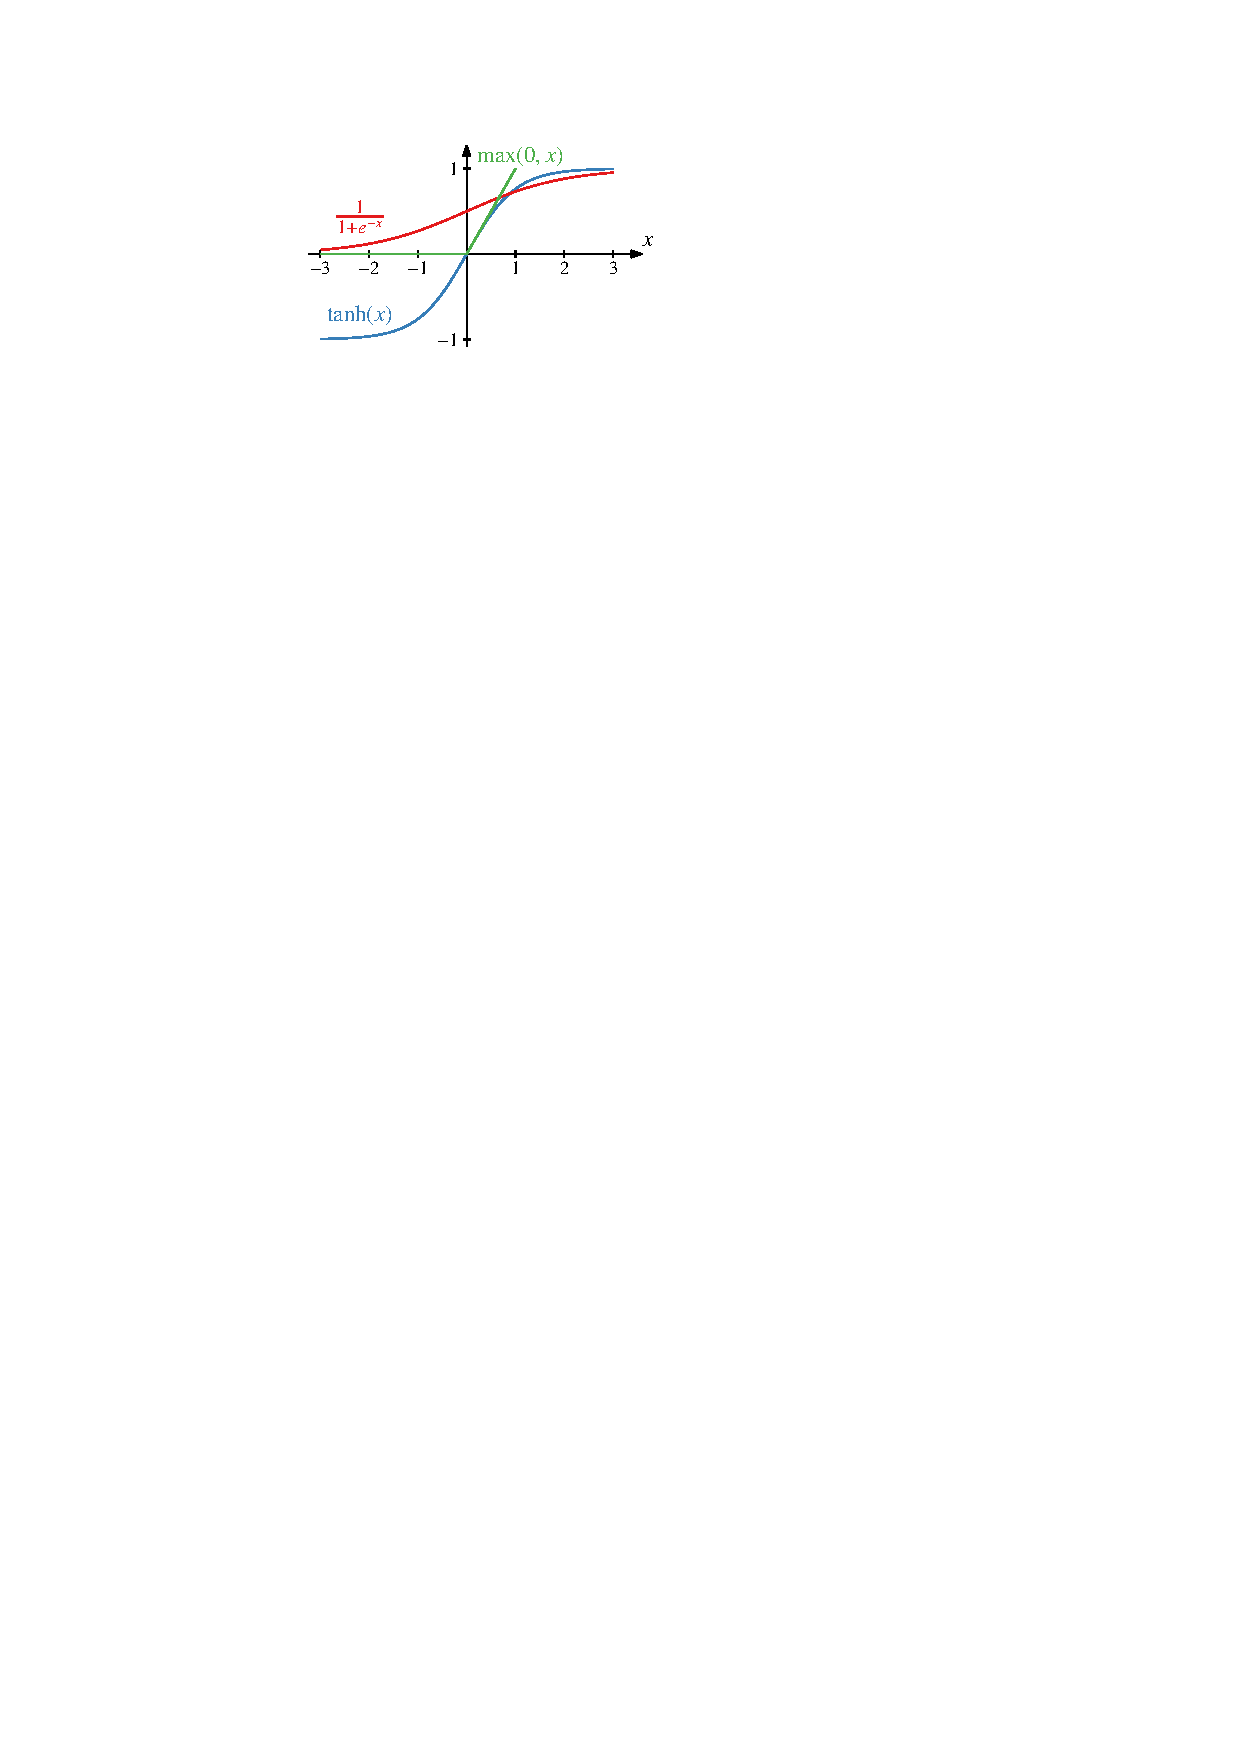
\includegraphics{./figures/theory/activation_functions.pdf}
    \subcaption{Commonly used activation functions for neural networks: logistic
      function (red), hyperbolic tangent (blue), and rectified linear unit --
      ReLU (green).}
    \label{fig:activation_functions}
  \end{subfigure}
  \caption{Feedforward neural network}
\end{figure}

\todo{$\varphi$ should be bold!}
Feedforward -> information flow from front to back.

An example of a simple feedforward neural networks is the multi-layer perceptron
consisting of a number of input neurons $\mathbf{x}$ that are used to feed the
discriminants to the network, a output layer with activation $\mathbf{y}$ and
several intermediate (hidden) layers connecting input and output layer. In
figure \ref{fig:multi_layer_perceptron} a multi-layer perceptron with a single
hidden layer is shown. Two layers of the network are connected by an affine
transformation $\mathbf{W}\mathbf{x} + \mathbf{b}$ and subsequent application of
an entry-wise activation function $\bm{\varphi}$ (commonly called dense or
densely-connected layers). The activations of the neurons in the hidden layer
$\mathbf{h}$ and the output layer $\mathbf{y}$ for the case depicted in figure
\ref{fig:multi_layer_perceptron} are given by:
\begin{align*}
  &\mathbf{h} = \bm{\varphi}_{\text{h}}(\mathbf{W}_{\text{hx}} \mathbf{x} + \mathbf{b}_{\text{h}})
  &\mathbf{y} = \bm{\varphi}_{\text{y}}(\mathbf{W}_{\text{yh}} \mathbf{h} + \mathbf{b}_{\text{y}}) \eqdot
\end{align*}
Generally the sizes of the hidden layers as well as the choice of the activation
functions are hyperparameters of the model. The exception is the size of the
input and output layer which is given by the number of discriminants and the
number of outputs respectively. Moreover the activation function of the final
layer is determined by the underlying task. For binary classification the
logistic function $\sigma(x) = (1 + \exp(-x))^{-1}$ is applied to a single
output neuron giving the probability of an observation being of the positive
class. For multi-class classification the number of output neurons is equal to
the number of classes and \emph{softmax}
\begin{align*}
  \varphi_i(\mathbf{x}) = \frac{e^{x_i}}{\sum_j e^{x_j}}
\end{align*}
is commonly chosen as the activation function, where $\varphi_i(\mathbf{x})$ is
the activation of the $i$-th neuron and $x_i$ the value of the neuron before
activation. The \emph{softmax} function ensures that the sum of activations in a
layer equals one, such that the activations can be interpreted as class
probabilities. Further activation functions that are commonly used for the
intermediate layers are depicted in figure \ref{fig:activation_functions}.

There are numerous different layers and ways to interconnect them, which allows
for high flexibility when building networks.

Training:
\begin{itemize}
\item Weight initialisation
\item Loss functions
\item Backpropagation \cite{lecun-backprop}
\item Mini-batch Gradient Descent
\item Cross-Validation
\end{itemize}

For the training of neural networks a loss function that penalises errors in the
model's predictions is needed. In $K$-class classification tasks a commonly used
loss function is the categorical cross-entropy. For an observation of true class
$k \in \{ 1, \dots, K \}$ with discriminants $\mathbf{x}$ and a model
$\mathbf{p}(\mathbf{x})$ with per-class probabilities $p_k$ it is defined as
\begin{align*}
  L\left(k, \mathbf{p}(\mathbf{x}) \right) = - \log\left( p_k(\mathbf{x}) \right) \eqdot
\end{align*}
For binary classification it is sufficient to give the predicted probability $p$
for the positive class (e.g.\ an observation being signal) such that the binary
cross-entropy can be written as
\begin{align*}
  L(p(\mathbf{x})) = -t \, \log(p(\mathbf{x})) - (1 - t) \, \log(1 - p(\mathbf{x})) \eqcomma
\end{align*}
where $t$ is the binary indicator of the true class (0 for the negative and 1
for the positive class). When looking at a subset of observations with event
weights $w_i$ the loss $\mathcal{L}$ is defined as
\begin{align*}
  \mathcal{L} = \frac{\sum_i w_i L_i}{\sum_j w_j} \eqcomma
\end{align*}
which in case of the cross-entropy can be interpreted as the negative
log-likelihood of the model parameters given the observed subset of data. These
losses expect networks to predict probabilities which can be met if the
activation function of the final layer is the logistic function or softmax (eq.
\ref{eq:softmax}). The training process minimises the loss $\mathcal{L}$
(maximises the likelihood) with respect to the model parameters, i.e.\ the
weights and biases of the network, given the observed training data.

\todo{Find proper references} \cite{esl}

Large penalties to predictions
that are far off. Its better to be sort of off instead of completely off.
Motivate where in this thesis these loss functions are used. Both losses are
also called 'Log Loss'. $p$ should be a class probability. Perfect classifiers
have loss of zero. Last layer in neural network effectively does logistic
regression on the intermediate representation created from the previous layers.

\section{Recurrent Neural Networks}
\label{sec:rnn}

Recurrent: If a network has one or more cycles, that is, if it is possible to
follow a path from a unit back to itself.

Physics motivation: Able to do regression and classification on sequences of
physics objects like tracks, clusters, particle flow objects etc..

\subsection{Fully-Connected RNN}
\label{sec:fully_connected_rnn}

% \textsc{Elman} network [Check Citation]\cite{elman}:
\textsc{Jordan} network \todo{look for citation}:
\begin{align*}
  \mathbf{c}_t &= \bm{\varphi}_{\text{c}}\left( \mathbf{W}_{\text{c}} \mathbf{x}_{t} + \mathbf{U}_{\text{c}} \mathbf{h}_{t-1} + \mathbf{b}_{\text{c}} \right) \\
  \mathbf{h}_t &= \bm{\varphi}_{\text{h}}\left( \mathbf{W}_{\text{h}} \mathbf{c}_{t} + \mathbf{b}_{\text{h}} \right)
\end{align*}
\todo{Should rename output $\mathbf{h}$ to $\mathbf{y}$ to be consistent.}
with trainable weights $\mathbf{W}$, recurrent weights $\mathbf{U}$ and biases $\mathbf{b}$.

Vanishing gradient problem: Applying the sigmoid function multiple times leads
to vanishing gradients (plot?).

\subsection{Long Short-Term Memory}
\label{sec:lstm}

\begin{figure}[t]
  \centering
  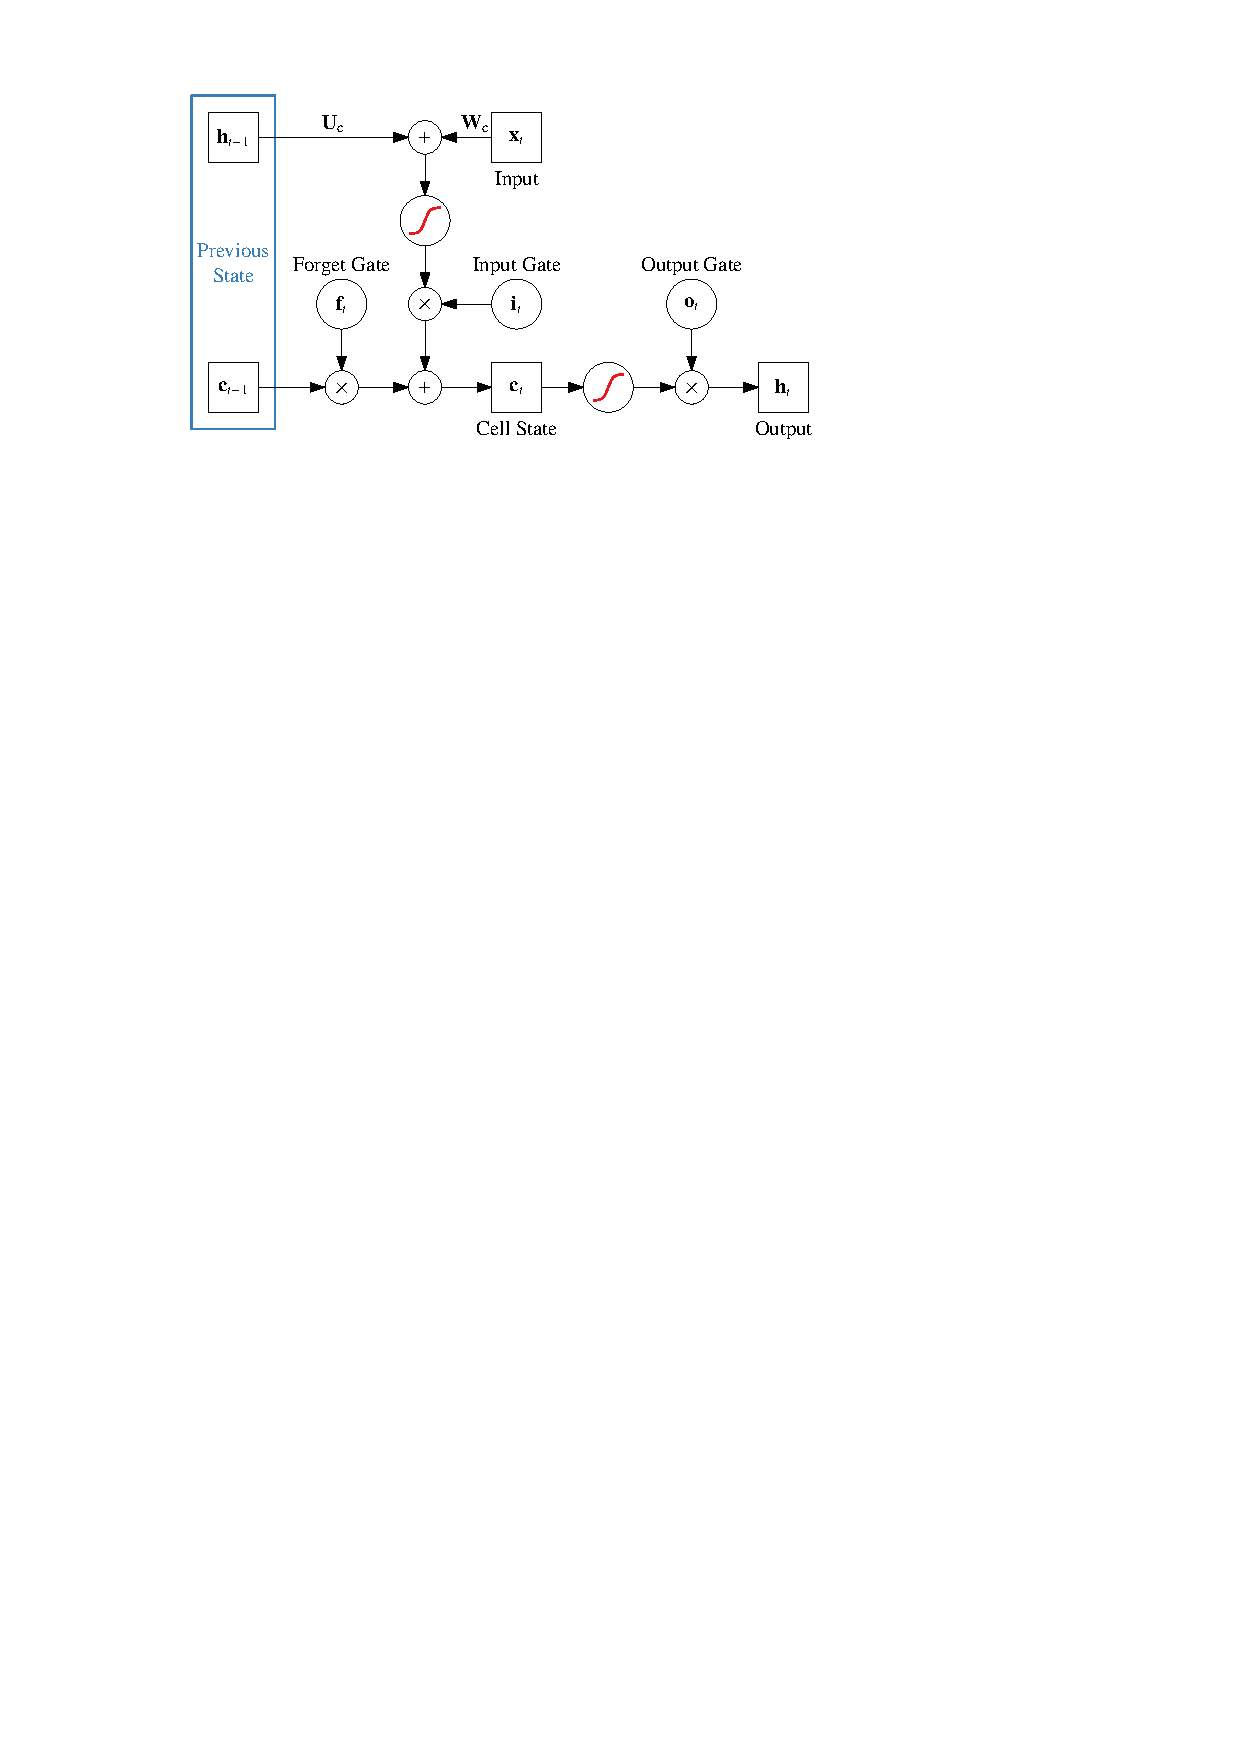
\includegraphics{./figures/theory/LSTM.pdf}
  \caption{Schematic description of a LSTM-cell.}
  \label{fig:schematic_lstm}
\end{figure}

[Check Citation]\cite{lstm}

Gate activations:
\begin{align*}
  \mathbf{f}_{t} &= \bm{\varphi}_{\text{g}}\left( \mathbf{W}_{\text{f}} \mathbf{x}_{t} + \mathbf{U}_{\text{f}} \mathbf{h}_{t-1} + \mathbf{b}_{\text{f}} \right) &
  \mathbf{i}_{t} &= \bm{\varphi}_{\text{g}}\left( \mathbf{W}_{\text{i}} \mathbf{x}_{t} + \mathbf{U}_{\text{i}} \mathbf{h}_{t-1} + \mathbf{b}_{\text{i}} \right) &
  \mathbf{o}_{t} &= \bm{\varphi}_{\text{g}}\left( \mathbf{W}_{\text{o}} \mathbf{x}_{t} + \mathbf{U}_{\text{o}} \mathbf{h}_{t-1} + \mathbf{b}_{\text{o}} \right)
\end{align*}
Cell state update:
\begin{align*}
  \mathbf{c}_{t} &= \mathbf{f}_{t} \circ \mathbf{c}_{t-1}
                   + \mathbf{i}_{t} \circ \bm{\varphi}_{\text{c}}(
                   \mathbf{W}_{\text{c}} \mathbf{x}_{t}+ \mathbf{U}_{\text{c}}
                   \mathbf{h}_{t-1} + \mathbf{b}_{\text{c}})
\end{align*}
Output:
\begin{align*}
  \mathbf{h}_{t} &= \mathbf{o}_{t} \circ \varphi_{\text{h}}(\mathbf{c}_{t})
\end{align*}

Stress that the gates depend on $x_t$ and $h_{t-1}$ via learn-able weights.
Therefore the inputting, outputting and forgetting is a learned process.

$\circ$: entry-wise product


Variables:
\begin{itemize}
\item $x_t$: input vector
\item $h_t$: output vector
\item $c_t$: cell state vector
\item $W$, $U$ and $b$: (recurrent -- $U$) weight matrices and bias vector
\item $f_t$, $i_t$ and $o_t$: gate vectors
  \begin{itemize}
  \item $f_t$: forget gate vector
  \item $i_t$: input gate vector
  \item $o_t$: output gate vector
  \end{itemize}
\end{itemize}

Activation functions:
\begin{itemize}
\item $\sigma_g$: element-wise sigmoid function (Gate activation -- recurrent
  activation)
\item $\sigma_c$: element-wise hyperbolic tangent (Cell activation -- recurrent
  activation)
\item $\sigma_h$: element-wise hyperbolic tangent (Output activation)
\end{itemize}


\section{Technical Setup}
\label{sec:tech_setup}

Frameworks used for this thesis (theano \cite{theano}, keras \cite{keras})

Optimiser: Adam

Masking layer


%%% Local Variables:
%%% mode: latex
%%% TeX-master: "mythesis"
%%% End:
